\def\stmt{$A$}
% \def\stmt{$\phi$}


\commentout{%oli-v1
	% The ability articulate a \emph{degree of confidence} is an important aspect of knowledge representation.
	The ability to articulate a \emph{degree of confidence} 
	% (or the opposite: a degree of uncertainty)
	is a critical aspect of representing knowledge.
	There are 
	% Correspondingly, there are
	many well-established ways to quantify (un)certinaty \parencite[\S2]{halpern2017reasoning},
		and chief among them is probability.
	While ``confidence'' can be coherently read in probabilistic terms,
		such usage may shadow another important concept.
	This paper details a different conception that arises when updating beliefs. 
	As we shall see, this notion of confidence
	complements traditional representations of uncertainty (such as probability), 
	and moreover unifies several different concepts across AI.
}

What should it mean to say that one has a high degree of confidence in a statement $\phi$?  It is often taken to mean that we think $\phi$ is likely. 
% This paper details a different conception that arises when updating beliefs. 
% As we shall see, this notion of confidence
% complements traditional representations of uncertainty (such as probability), 
Here we argue that there is a related but more useful conception of confidence that arises when updating---one that complements likelihood and, moreover, unifies several different concepts in the literature.
% Here we argue that there is a related but more useful way of defining confidence, which complements notions like probability and, moreover, unifies several different concepts in the literature.

% For us, confidence is a measure of trust (in incoming information), rather than of likelihood (of hypothetical information). 
% For us, confidence (in an input $\phi$) is a measure of \emph{trust}, rather than of likelihood; it quantifies seriously to take $\phi$ in updating one's beliefs.
%
%joe1:
% For us, the degree of confidence in $\phi$ is a measure of the degree
% to which we \emph{trust} $\phi$,
% rather than of the likelihood of $\phi$.  We formalize this by taking
% the degree of confidence to represent how seriously to take $\phi$
% when updating beliefs.
%
%oli1: with reference to your rewrite (above): I don't like the way the grammar 
% worked out; my lead-in "for us" muddies the "our confidence" part 
% that you wrote. Let me try to clean it up. 
%
For us, confidence is a measure of \emph{trust}, rather than likelihood.
In particular, the {degree of confidence} that one has in a piece of information $\phi$
%is a number  $\chi \in [\bot,\top]$ that 
quantifies how seriously to take $\phi$ in updating one's beliefs. 
%oli1:
% In the below, I replaced "0" and "1" with "no" and "full" because
% I want don't want to lock in the range [0,1] at this level of generality.
% More importantly, the second part about "taking \phi to be true" doesn't
% make as much sense in general, so I rephrased it.
%
% Thus, if we learn $\phi$ but have confidence 0 in it, it should not
% affect our beliefs at all, while if we have confidence 1 in $\phi$, we
% should update our beliefs by taking $\phi$ to be true; in a
% probabilistic setting, this amounts to conditioning on $\phi$. 
%
% Thus,
So at one extreme,
if we observe $\phi$ but have no confidence in it, 
% it should not affect our beliefs at all;
we should not change our beliefs at all;
at the other, if we have full confidence in $\phi$,
 we should fully incorporate it into our beliefs.
 
% , in some sense.
% In the setting where, our beliefs is a probability measure $\Pr$, and $\phi$ is an event, 
% In a probabilistic setting, we can capture an intermediate degree of
% If our belief state is a probability measure $\Pr$ and $\phi$ is an event, for example, then fully incorporating $\phi$ amounts to conditioning $\Pr$ on it.
Suppose, for example, that 
% For example, if
our belief state is a probability measure, and $\phi$ is an event. 
In this setting, 
a full-confidence update amounts to conditioning on $\phi$, after which $\phi$ has probability 1 and cannot be further incorporated.
%oli1: changed from "the obvious way" to "an obvious way"
% In a probabilistic setting, we can capture an  intermediate degree of confidence by interpolating in the obvious way:
In this case,
% we can also capture intermediate degrees of confidence in an obvious way:
there is also an obvious way to describe intermediate degrees of confidence:
if we learn $\phi$ with confidence
%oli1: now adding range here
% $\alpha$
$\alpha \in [0,1]$
% and start with a prior probability $\Pr$, then we end up with the
and start with prior probability $\Pr$, then we might end up with the
posterior $(1-\alpha)\Pr + \alpha (\Pr\mid \phi)$.
%
Thus, having high confidence in $\phi$ leads to posterior beliefs that give $\phi$
high
%oli1: I've seen a lot of statistics people make a big fuss about
% this being the wrong usage of the word "likelihood", which I've been
% told applies to evidence that is being conditioned on, and not to 
% events whose probability we're querying.  Now that we have a
% probability in scope, I'd prefer to avoid this fight by just saying:
%likelihood.
probability.
% But confidence and probability are not always so tightly coupled.
Still, confidence and probability are quite different in general.
% 
%oli1: the context here has been stripped; we're now missing how it might be possible to learn \phi with low confidence if we already assign it high probability.
% If we start out with a prior that gives $\phi$ high likelihood, and learn $\phi$ with low confidence, our posterior beliefs still give $\phi$ high likelihood.  
% We might also have a great deal of confidence in an observation of $\phi$  despite having a low prior belief in $\phi$.
If an untrusted source tells us $\phi$ which we already happen to believe, 
then our prior gives $\phi$ high probability, but we learn $\phi$ with low confidence, and then our posterior beliefs still give $\phi$ high probability.  
% Confidence is even easier to distinguish from prior probability: 
Confidence and prior probability are even more independent: 
if we learn a surprising fact $\phi$ from a trusted source, we have high confidence in $\phi$ despite it having low prior probability.
% This leads to an important observation: one's confidence in $\phi$ is not a feature of one's prior probability at all.


\commentout{
	In this context, 
	the confidence $\chi \in [0,1]$ has a clear interpretation as the ``fraction of the way towards full incorporation'',
	but in others,
	it may be 
	less clear what a number on this scale (say, $\chi{=}0.7$) means.
	% there is still a natural path from distrust to complete trust that is parameterized differently.
	% In other cases, there are other more natural ways to articulate one's confidence.
}


But confidence can be applied far more broadly.
Consider a neural network, whose ``belief state'' is a setting of weights.
	% which are updated when given a training point.
% As it sees each training point, it updates its weights. 
% Modern learning algorithms do not take any individual point too seriously; each training point $x$ changes the weights incrementally, and alone may not even be enough for the network to classify that point correctly.
%oli1:adding, per our discussion
For definiteness, suppose we are talking about a classifier, so that there is a function $f : \Theta \times X \to \Delta Y$, that, when supplied a setting of the network weights weights $\theta \in \Theta$, and an input $x \in X$, outputs a distribution $f_\theta(x)$ over possible class lables $Y$. 
Modern learning algorithms (like gradient descent) make small incremental changes to the weights, and so updating with a labeled training example $\phi = (x,y)$ does not ensure that $f_\theta(x)$ is of high probability. 
% does not guarantee that the resulting network handles $x$ correctly. 
% In other words, the algorithm does not take any individual point too seriously.
In other words, such algorithms 
(in contrast to their historical counterparts \parencite{conjunctions}) 
do not take any one encounter with a training example too seriously.
% So, in contrast with conditioning, there is a significant difference betwen cycling through the training data once, and doing so many times.
This distrust of any individual observation is arguably what makes the training process so robust to noisy and conflicting observations.
\commentout{
	As a result,
	there is a significant difference between going through the training data once
	 % (a single epoch)
	\unskip, and doing so many times.}
Nevertheless, the weights do eventually converge if we repeatedly train on $x$, 
% which is a natural notion of 
% % ``fully incorporating $x$''---%
% full incorporation---%
an extreme action that is only appropriate if we trust $x$ completely.
% At the other extreme, if we had no trust in $x$, we could ignore it leaving our weights unchanged. 
% In this context, 
% Once again we have two extremes:
% Depending on our confidence, 
% How we ought to treat $x$ 
% What we ought to do depends on our confidence.
% At one extreme, we have no trust in $x$ and should ignore it, leaving weights unchanged; at the other, we trust $x$ completely, we should adopt the weights that arise in the limit of infinite training. 
% Moreover, this sequence of incremental updates (roughly) describes a path between the two extremes.%
Moreover, this sequence of incremental updates describes a path, from the opposite, low-confidence extreme of ignoring $x$.%
	\footnote{This path can be made into a continuous path by interpolating with a line segment, and made smooth in the limit of small step sizes; we will deal with both constructions in \cref{sec:project-additive}.}
Note that the relevant geometry here is not just the geometry of the weight space, but also that induced by the architecture and the loss function.
% As we will see in \cref{sec:loss-repr}, such 
% We have now seen a new way of quantifying confidence: the number of training iterations.
% The number of training iterations a different way of quantifying confidence.  
It is not so clear that a fraction of the way to completion (say 0.7) is as meaningful here as it was before (and it would be difficult to recognize that point in any case),
but we now have a different way to quantify confidence: the number of training iterations. 
% It turns out that in general, there are close relationships 

While there are some good reasons to prefer the first approach, 
the second one is more general. 
We can treat the example in this way: once we fix a ``unit confidence'', say $\chi=0.01$, a sequence of $n$ unit updates is equivalent to a single one of confidence $\chi= 1-(0.99)^n$. 
This general idea can be cleaned by appeal to differential geometry.
Specifically, we can take a limit

Moreover, in the case where belief states are Dempster-Shafer belief functions, 
and inputs are simple support functions, this measure of confidence is what Shafer calls the \emph{weight of evidence} \parencite{shafer1976mathematical}.

the updating process can be written as a vector field.




% natural measure of confidence that works in all cases,
% which 
% It turns out that there is a natural way of measuring confidence in all cases of interest, based on differential geometry of belief space. 
% Furthermore, in the case where belief states are Dempster-Shafer belief functions, 
% and inputs are simple support functions, this measure of confidence is what Shafer calls the ``weight of evidence''.
%% TODO: Shafer


%%%%% PARAGRAPH ON MANY DIFFERENT VIEWPOINTS
% Linear interpolation, however, is just the tip of 
% At the heart of our paper is a hierarchy 



\begin{figure}
\centering
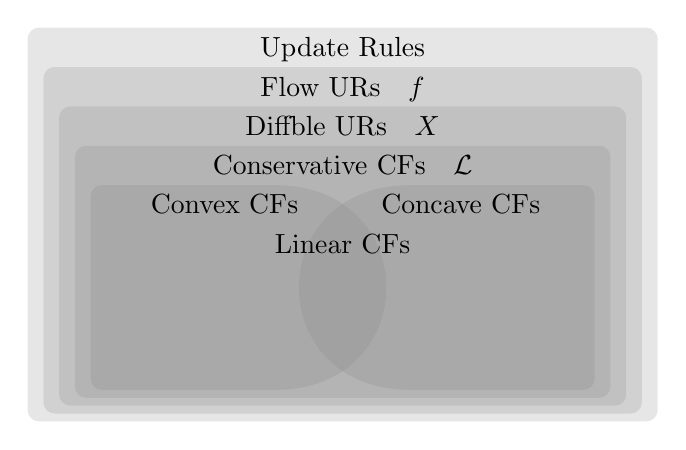
\begin{tikzpicture}
	\begin{scope}[fill=gray,fill opacity=0.2,rounded corners=4px]
		\fill (0,0) rectangle (8,5); % URs (Full Updates)
		\fill[] (0.2,0.1) rectangle (7.8,4.5); % Flow URs (Flows)
		\fill[] (0.4,0.2) rectangle (7.6,4.0); % Diffble URs (Vec Field)
		\fill[] (0.6,0.3) rectangle (7.4,3.5); % Conservative URs 
		\fill (0.8,0.4) -- (0.8, 3.0) -- (3, 3.0)
		 	to[out=0,in=0,looseness=2] (3,0.4) --cycle; % CONVEX
		\fill (7.2,0.4) -- (7.2, 3.0) -- (5, 3.0)
		 	to[out=180,in=180,looseness=2] (5,0.4) --cycle; % CONCAVE
	\end{scope}
	\begin{scope}[anchor=north]
		\node at (4.0, 5.0) {Update Rules};
		\node at (4.0, 4.5) {Flow URs~~~$f$};
		\node at (4.0, 4.0) {Diffble URs~~~$X$};
		% \node at (4.0, 3.5) {Conservative CFs~~~$\mathcal L$};
		\node at (4.0, 3.5) {Conservative CFs~~~$\mathcal L$};
		\node at (2.5, 3.0) {Convex CFs};
		\node at (4.0, 2.5) {Linear CFs};
		\node at (5.5, 3.0) {Concave CFs};
	\end{scope}
\end{tikzpicture}
\caption{%
	A map of different kinds of commitment functions and their representations.}
\end{figure}


% It is not always most natural for confidence to range between zero and one. 
% But there are many instances in which 
% However, there is a more universal representation of it in $[0, \infty]$

% While probability ranges from untenable (0) to undeniable (1),
% confidence ranges from completely untrustworthy $(\bot)$ to fully trusted ($\top$).




\commentout{
	\subsection{Other Conceptions of Confidence.}

	\textbf{Probability.}
	% Probability is a numerical scale that ranges from untenable (0) to undeniable (1).
	% No number on this scale is truly neutral.
	% One of the biggest shortcomings of probability is its inability to represent a truly neutral attitude towards a proposition.
	Some people do use ``confidence'' to mean the same thing as probability. When they say they have low confidence in $\phi$, they mean that they think $\phi$ is unlikely.

	One of the biggest shortcomings of probability is its inability to represent a truly neutral attitude towards a proposition.
	%  probability of $\frac12$ .
	% This shortcoming has perhaps been the primary selling point of many alternatives to probabiltiy, such as Dempster-Shafer Belief functions.
	A value of $\frac12$ may be equally far from zero as it is from one, but is by no means a neutral assessment in all cases: hearing that your favored candidate has a 50\% chance of winning is big news if a win was previously thought to be inevitable.
	For this reason, telling someone the odds are 50/50 is quite different from saying you have no idea.
	% By contrast, zero confidence represents a truly neutral stance; a statement with zero confidence has no effect.
	By contrast, zero confidence represents something truly neutral:
		a statement made with zero confidence does not stake out a claim, and
		a statement recieved with zero confidence does not affect the recipient's beliefs.
	Nevertheless, in some contexts, we will see that confidences correspond to to probabilities.

	\textit{Opacity.} To use a graphical metaphor, think of certainty as black or white.
	Probability describes shades of gray, while confidence describes opacity.
	If we are painting with black and start with a white canvas, there is a precise correspondence between the opacity and the resulting shade of gray.

	\textbf{Upper and Lower Probabilities.}
	Upper and lower probabilities can describe a neutral attitude towards a proposition, but they are not really a specification of trust, but rather a direct specification of a belief state.
	It isn't immediately clear how to use these representations of uncertainty to update, and they're a little too complex to function effectively as the primitive measure of trust that we're after.


	\textbf{Shafer's Weight of Evidence.}
	Shafer's ``weight of evidence'' is precisely the same concept we have in mind.
	Our analysis precsely reduces to his, in the setting where belief states are Belief functions (which generalize probabilities, but not, say, neural network weights), and observations are events.
	% This paper can be a generalization of Shafer's ``weight of evidence'' to a broader class of settings, where one might have very different belief states and observations.
	Thus, this paper can be viewed as generalizing this concept to a broader class of settings, without requiring that one adopt Shafer's conception of a belief state or an observation.


	\textbf{Variance and Entropy.}
	The inverse of variance, sometimes known as precision,
		is also commonly used to measure confidence.
	If a sensor is unreliable and can give a range of answers, the variance of the estimate is a very common way of quantifying this reliablility.
	If measurements have zero variance, in some sense one has absolute confidence ($\top$) in the sensor. If measurements have infinite variance, then in some sense one has no confidence in the sensor, since individual samples convey no information about the true value of the quantity measured.
	As with probability, inverse variance will coincide with confidence in some settings; we will see how in \cref{sec:variance}.

	Entropy, like variance, is a standard way of measuring uncertainty, and in some settings, confidence coincides with entropy (see \cref{sec:entropy}).
	The assumption underlying both approaches is that there's some ``true'' value of the variable, and that the randomness is epsistemic (due to sensor errors) rather than aleotoric (inherrent in the quantity being measured).

	\textbf{Confidence Intervals and Error Bars.}
	Another notion of the word ``confidence'' comes from the term ``confidence interval''.
	This concept arises in settings involving a probability distribution $\Pr(X)$ over a metric space $X$, typically $X = \mathbb R$.
	A 95\% confidence interval is the (largest) ball containing 95\% of the probability, and its size is a geometric measurement of how .
	This intuition behind this reading of the word confidence is the same as
}
